\graphicspath{{main/implementation/graphics}}

\section{Testing}

% Some text

% If you are developing software or hardware, you must test it.  This section should explain how your work will be (or has been) tested.

% You should have a test plan at the very least (full details of it and its results if required can go in an appendix).  Ideally, you will have automated tests for any software you build.  You will also define user acceptance tests, or something similar which can be used to determine whether your output meets the requirements stated earlier.  Explain how and when the tests should be conducted

% Maybe also mention software quality here, following do178c etc.

% Test driven development

\subsection{Unit Tests}

To complement the end-to-end experiments for testing real-time behaviour, unit-tests were made across the software infrastructure packages. These were designed to find small software bugs in the implementation during development.

An example unit test is shown in \autoref{lst:unitTestCommunication}. This was used to test that bad communication messages were rejected by the communication client library. The test mocked the communication socket so that false data could be sent through it.

\hfill

\begin{lstlisting}[caption=Example unit test (communications), label={lst:unitTestCommunication},captionpos=b]
#[test]
fn test_communication_zero_length() {
    setup();

    let (socket, child_socket) = UnixStream::pair().unwrap();
    socket.set_nonblocking(true).unwrap();
    child_socket.set_nonblocking(true).unwrap();

    let mut manager = Manager::new(child_socket);

    // put bad data on socket
    let mut stream = &socket;
    let length_buf = [0, 0, 0, 0];
    stream.write_all(&length_buf).unwrap();

    manager.run();

    let message = manager.get_message(1);
    assert_eq!(message, None);
}
\end{lstlisting}

Using the unit tests, code coverage reports were generated. These expressed the percentages of the different sections of the code that were executed during the unit tests. The \verb|llvm-cov| reports were created using \verb|cargo-llvm-cov| \autocite{endoTaikieCargollvmcov2024} and are shown in \autoref{fig:tetsingCoverage}.

Function coverage simply counts the number of times a function has been executed. This also includes inline functions. Line coverage checks how many times each line has been executed. Region coverage evaluates the number of times a subdivision of a function has been executed. For example, true/false control flow \autocite{llvmSourcebasedCodeCoverage2024}.

\clearpage

Each coverage metric is important for gaining a heuristic view of what percentage of the source code has been tested. This is specifically useful for software certification. DO-178B/C at the highest safety classification (DAL A) expects functions, lines, blocks and conditions coverage to be near 100\% \autocite{ibmHowCodeCoverage2022}. Currently Rust does not support condition coverage with llvm-cov. Condition coverage checks that all combinations of branches have been executed \autocite{llvmSourcebasedCodeCoverage2024}.


\begin{figure}[ht]
  \centering
  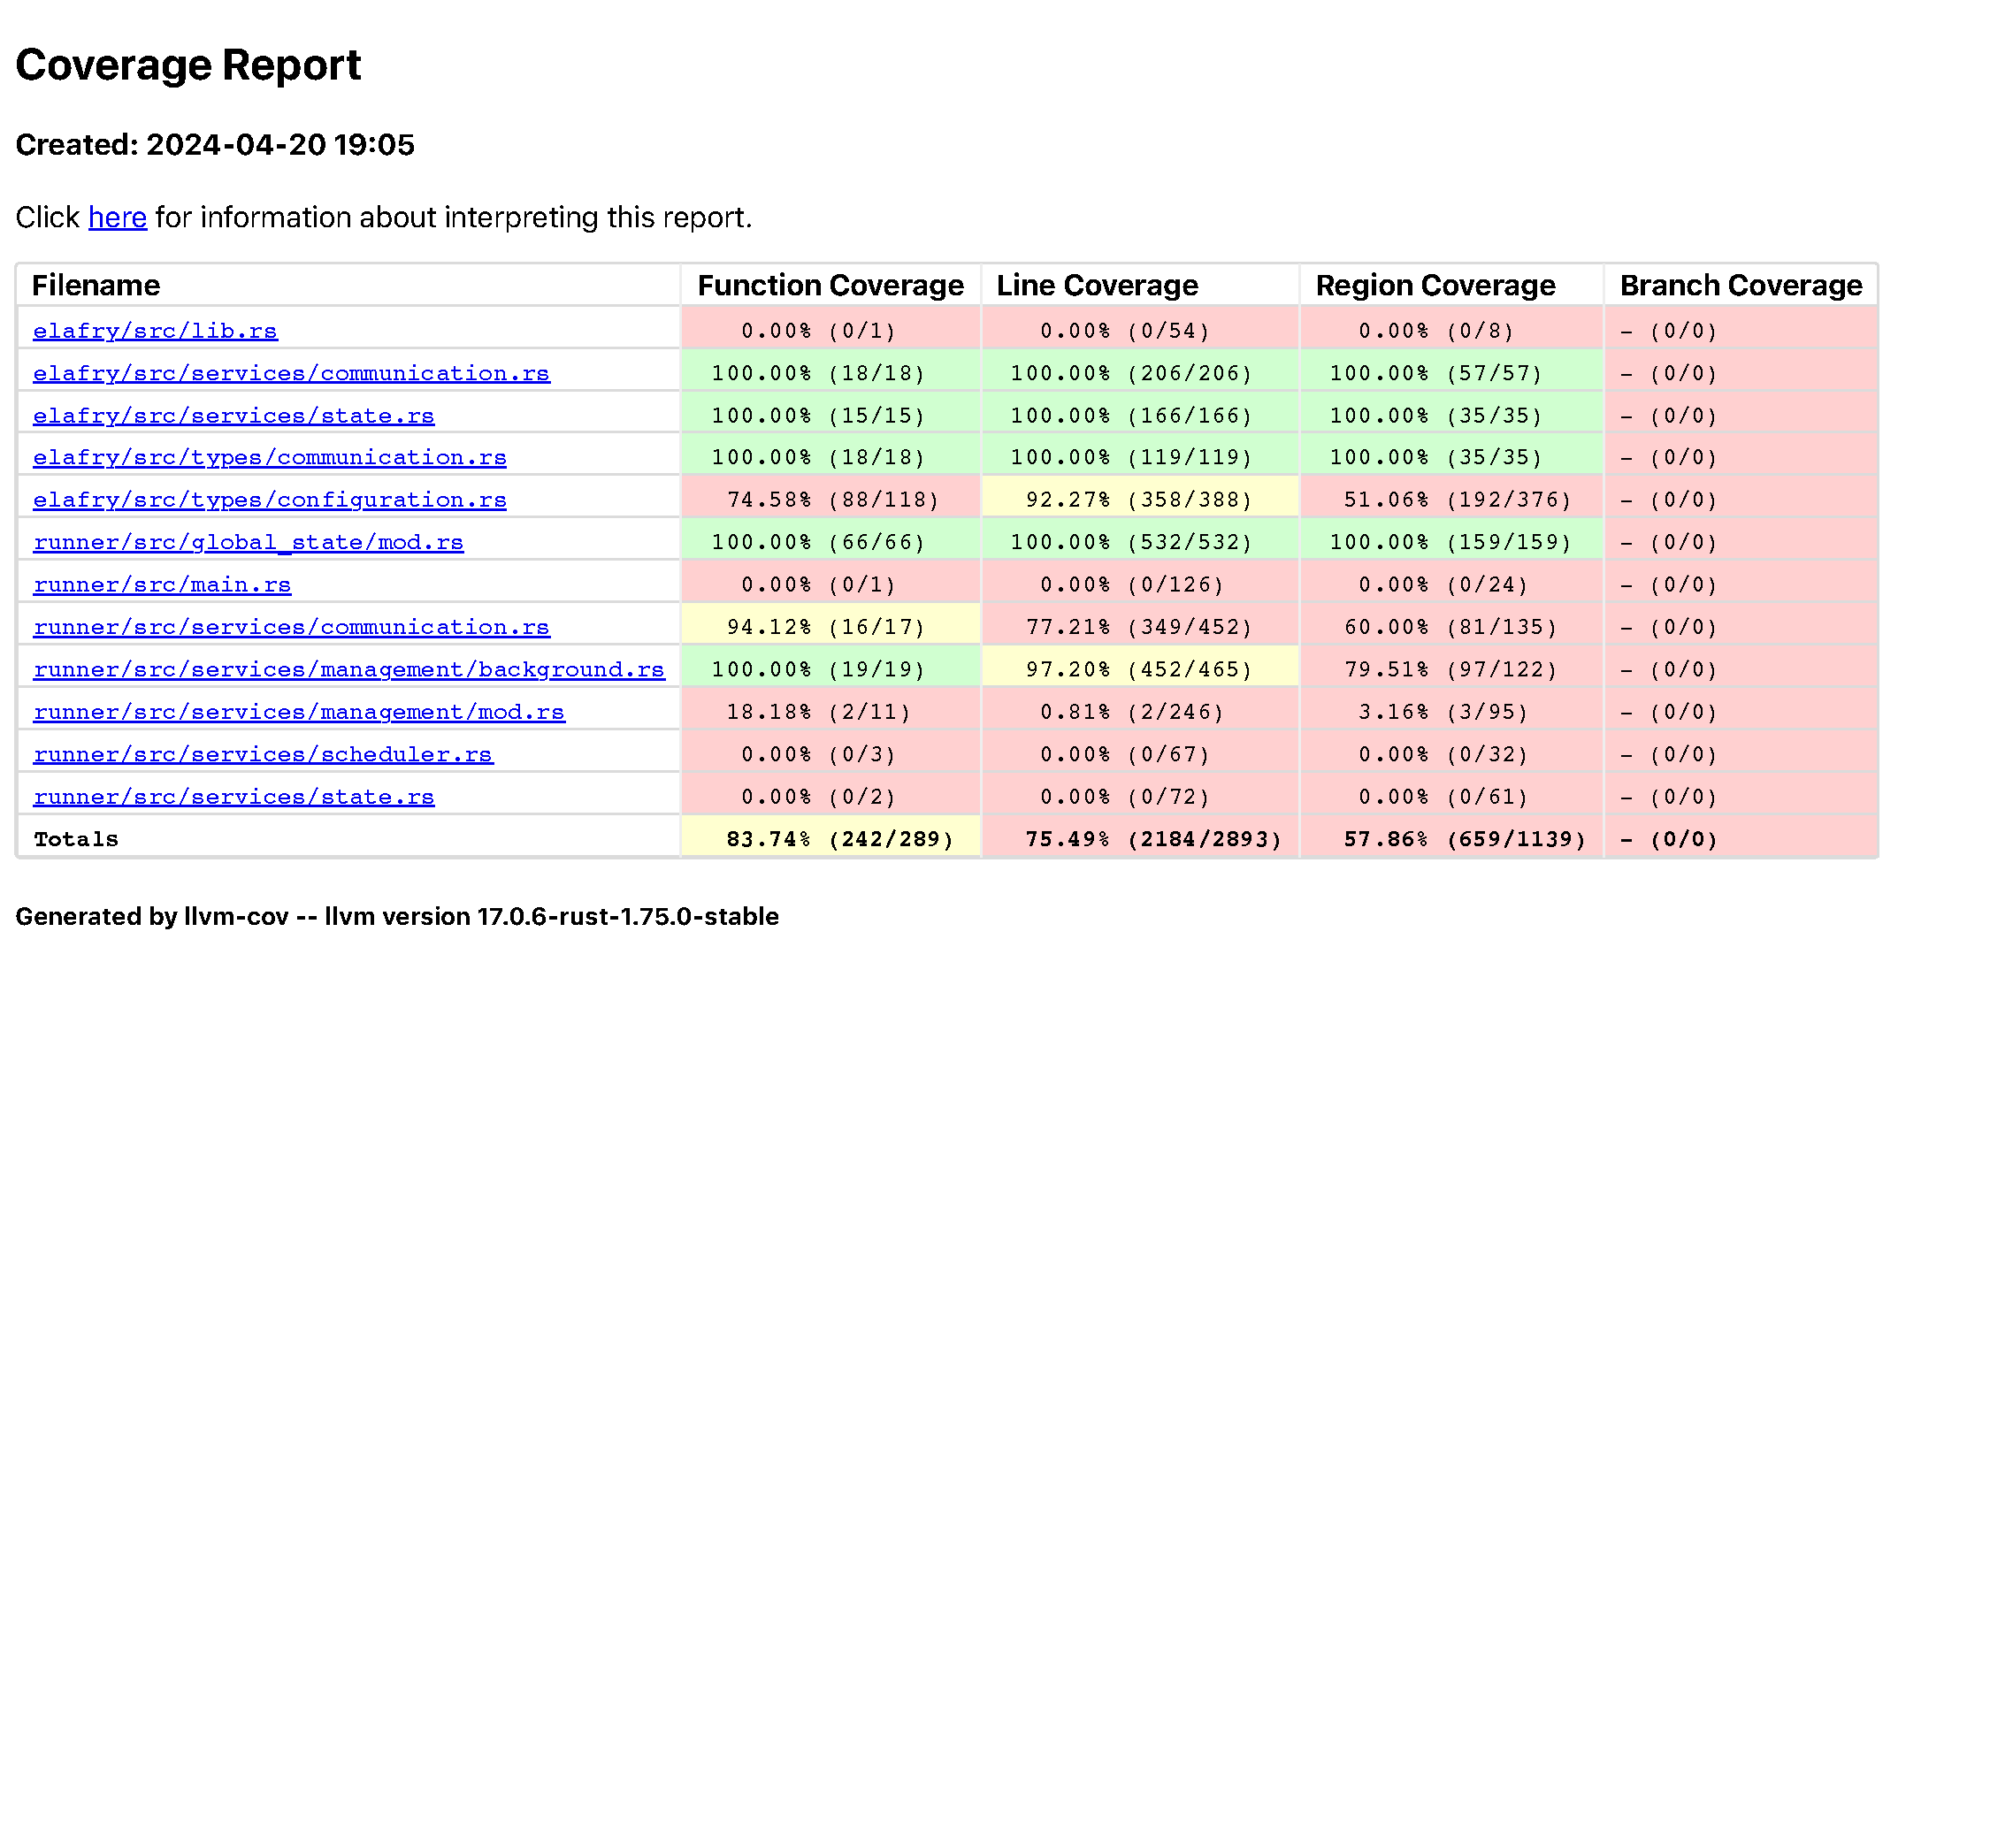
\includegraphics[width=\textwidth, clip, trim=0.1cm 16.9cm 2cm 0.5cm]{coverage.pdf}
  \caption[Code coverage report (llvm)]
  {Code coverage report (llvm)}
  \label{fig:tetsingCoverage}
\end{figure}

During development it was challenging producing the unit tests for every function as the software infrastructure mainly interacted with components. Hence, these components had to be mocked to simulate the usual data flow. 

Packages that were entirely internal were easy to create unit tests for because they didn't interact with the operating system. For example, \verb|global_state| achieved 100\% code coverage as this class only contained functions that modified the program's local state. Given more development time, the unit test could be expanded for complete code coverage.

% \begin{table}[ht]
%   \centering
%   \caption{Caption}
%   \label{tab:table1}
%   \begin{tabular}{l|ccc|c}
%     \toprule
%      \thead{Requirements} & \rothead{Unit Tests} & \rothead{End-To-End Tests} & \rothead{Opinion} & \rothead{Complete}  \\
%     \midrule

%     \ref{item:reqSIComp} & $\checkmark$ & & & \\
%     \ref{item:reqSICompStartStop} & $\checkmark$ & & & \\
%     \ref{item:reqSICompSched} & & $\checkmark$  & & \\
%     \ref{item:reqSIMess} & $\checkmark$ & & & \\
%     \ref{item:reqSIMessRoute} & $\checkmark$ & & & \\
%     \ref{item:reqSIMessRouteChange} & $\checkmark$ & & & \\
%     \ref{item:reqSIState} & $\checkmark$ & & & \\
%     \ref{item:reqSIStateSave} & $\checkmark$ & & & \\
%     \ref{item:reqSIStateRestore} & $\checkmark$ & & & \\
%     \ref{item:reqSIStateTransform} & $\checkmark$ & & & \\
%     \bottomrule
% \end{tabular}
% \end{table} 